\documentclass[14pt,a4paper]{article}
\usepackage{mathtools}
\usepackage{amsmath}
\usepackage{bigints}
\usepackage{mathrsfs}
\usepackage{setspace}
\usepackage{amsfonts}
\usepackage{geometry}
\geometry{a4paper, total = {210mm,297mm},left=35mm, right=25mm,top=25mm,bottom=25mm}
\usepackage{xcolor}
\usepackage{mcode}
\usepackage{listings}
\lstset{basicstyle = \fontsize{12}{13} \selectfont\ttfamily}
\usepackage{graphicx}


%Begin document - Numerical Analysis - Homework 1

\begin{document}
\label{cover}
\begin{center}
	\vspace*{3cm}
	\large{\textbf{MATH/CS 5466 NUMERICAL ANALYSIS \\ Homework 1}}
	\vfill
	\textbf{Luan Cong Doan} \\ luandoan@vt.edu
	%\vfill
%	Department of Mechanical Engineering \\ Virginia Polytechnic Institute and State University
	\vfill
	\today
\end{center}
\pagebreak

\label{Answer Sheet}
\label{Numerical Exercise}
\doublespacing
\large\textbf{Problem 1.} This problem addresses the $\xi = \xi(x)$ term that appear in the formula: 
\hspace*{4cm} $$ f(x) - p_n(x) = \dfrac{f^{n+1}(\xi(x))}{(n+1)!}\sum_{j=0}^{n}(x-x_j) $$ 
\begin{enumerate}
	\item Write down the linear interpolant $p_1(x)$ for the function $f(x) = x^3$ at the interpolant points $x_0 = 0$ and $x_1 = b$: \\
		We have: \hspace{1cm} $f(x_0) = 0^3 = 0$ \hspace{2cm} $f(x_1) = b^3$\\
		\hspace*{2cm} $p_1(x) = p_0(x) + c_1q_1(x_1)= f(x_0) + \dfrac{f(x_1) - f(x_0)}{x_1 - x_0} (x - x_0) $\\
		\hspace*{6.45cm} $ = 0^3 + \dfrac{b^3 - 0^3}{b - 0}(x-0) $ \\
		\hspace*{6.45cm} $ = b^2x $
	
		According to Theorem 1.3 in course notes we have:
		\hspace*{2cm} $$ f(x) - p_n(x) = \dfrac{f^{(n+1)}(\xi(x))}{(n+1)!}\prod_{j=0}^{n}(x-x_j)$$
		Applied above Theorem for $n =1$ we have:
		\hspace*{1cm} $$ f(x) - p_1(x) = \dfrac{f^{(2)}(\xi(x))}{2!}\prod_{j=0}^{1}(x-x_j)$$
		\hspace*{2cm} $ \Leftrightarrow x^3 - b^2x = \dfrac{6(\xi(x))}{2}(x-x_0)(x-x_1)$ \\
		\hspace*{2cm} $ \Leftrightarrow x(x-b)(x+b) = 3(\xi(x))x(x-b) $\\
		\hspace*{2cm} $ \Leftrightarrow (x+b) = 3(\xi(x))$ \\
		\hspace*{2cm} $ \Leftrightarrow \xi(x) = \dfrac{(x+b)}{3} $ 
		
	\item Write down the linear interpolant $p_1(x)$ for the function  $f(x) = 1/x$ at the interpolation points $x_0 = 1$ and $x_1 = 2$:\\
		We have: \hspace{1cm} $ f(x_0) = \dfrac{1}{1} = 1$ \hspace{1cm} $f(x_1) = \dfrac{1}{2}$ \\
		\hspace*{2cm} $p_1(x) = p_0(x) + c_1q_1(x_1)= f(x_0) + \dfrac{f(x_1) - f(x_0)}{x_1 - x_0} (x - x_0) $\\
		\hspace*{6.45cm} $ = 1 + \dfrac{\dfrac{1}{2} - 1}{2 - 1}(x-1) $ \\
		\hspace*{6.45cm} $ = -\dfrac{x}{2} + \dfrac{3}{2} $\\
		Applied above Theorem for $n =1$ with $f^{(2)}(\dfrac{1}{x}) = \dfrac{2}{x^3}$ we have:\\
		\hspace*{2cm} $ \dfrac{1}{x} - \left(-\dfrac{x}{2} + \dfrac{3}{2}\right) = \dfrac{\dfrac{2}{(\xi(x))^3}}{2}(x-1)(x-2)$ \\
		\hspace*{2cm} $ \Leftrightarrow \xi^3(x)(x^2 - 3x +2) = 2x(x-1)(x-2)$ \\
		\hspace*{2cm} $ \Leftrightarrow \xi^3(x) = 2x$\\
		\hspace*{2cm} $ \Leftrightarrow \xi(x) = \sqrt[3]{2x} = (2x)^{\dfrac{1}{3}}$ \\
		We have: $\xi'(x) = \dfrac{2}{3}(2x)^{-\dfrac{2}{3}} \Rightarrow \begin{cases} \xi'(x) = 0 & \quad  x =0 \\ \xi'(x) > 0 & \quad \forall x \neq 0 \end{cases} $ \\
		\hspace*{1cm} $ \Rightarrow \xi(x)$  is increasing in [1  2] so:\\
		\hspace*{2cm} $min_{1 \leq x \leq 2}\xi(x) = \xi(1) = (2.1)^{\dfrac{1}{3}}= 1.2599$ \\
		\hspace*{2cm} $max_{1 \leq x \leq 2}\xi(x) = \xi(2) = (2.2)^{\dfrac{1}{3}} = 1.5874$ 
\end{enumerate}

\large\textbf{Problem 2.} Recall for $\textbf{A} \in \mathbb{C}^{n \times n}$, the linear system $\textbf{A}\textbf{c} = \textbf{f}$ has a unique solution for any \textbf{f} provided Ker(\textbf{A}) = \{0\}, where Ker(\textbf{A}) denotes the kernel (null space) of \textbf{A}. \\
If the kernel of \textbf{A} is larger, i.e., if there is a nonzero vector $\textbf{z} \in $ Ker(\textbf{A}), then there are two possibilities: \\
	$\bullet$ If \textbf{f} $\notin$ Ran(\textbf{A}) then there is \textit{no solution} \textbf{c} to the linear system \textbf{Ac = f}. \\
	$\bullet$ If \textbf{f} $\in$ Ran(\textbf{A}), then there are \textit{infinitely many solutions} to the linear system \textbf{Ac = f}. In particular, if $\hat{\textbf{c}}$ satisfies \textbf{A}$\hat{\textbf{c}}$ = \textbf{f}, then there any \textbf{c} of the form \textbf{c} =  $\hat{\textbf{c}}$ + $\gamma$\textbf{z} is also a solution, where $\gamma$ is an arbitrary constant. 
	
	\begin{enumerate}
		\item Suppose we wish to construct a polynomial $p_5 \in \mathcal{P}_5$ that interpolates a function $f \in \mathbb{C}^2[-1, 1]$ in the following manner: $p_5(-1) = f(-1)$; \hspace{0.2cm} $p'_5(-1) = f'(-1)$;\\ $p_5(0) = f(0)$; \hspace{0.2cm} $ p"_5(0) = f"(0)$; \hspace{0.2cm} $p_5(1) = f(1)$; \hspace{0.2cm} $p'_5(1) = f'(1)$.  \\
		Write down a linear system to determine the coefficients $c_0, ..., c_5$ for $p$ in the monomial basis: $p_5(x) = c_0 + c_1x + c_2x^2 + c_3x^3 + c_4x^4 + c_5x^5$.\\
		As defined above, we have: $x_0 = -1; x_1 = 0; x_2 = 1$ and:\\
		\hspace*{2cm} $p'_5(x) = c_1 + 2c_2x + 3c_3x^2 + 4c_4x^3 + 5c_5x^4$\\
		\hspace*{2cm} $p"_5(x) = 2c_2 + 6c_3x + 12c_4x^2 + 20c_5x^3$\\
		(1). $ p_5(x_0) = c_0 + c_1x_0 + c_2x_0^2 + c_3x_0^3 + c_4x_0^4 + c_5x_0^5 = f(x_0)$\\
		\hspace*{1.9cm} $ \Leftrightarrow c_0 + c_1(-1) + c_2(-1)^2 + c_3(-1)^3 + c_4(-1)^4 + c_5(-1)5 = f(-1)$\\
		\hspace*{1.9cm} $ \Leftrightarrow c_0 - c_1 + c_2 - c_3 + c_4 - c_5 = f(-1)$\\
	%	\pagebreak
		(2). $p'_5(x_0) = c_1 + 2c_2x_0 + 3c_3x_0^2 + 4c_4x_0^3 + 5c_5x_0^4 = f'(x_0)$\\
		\hspace*{1.85cm} $ \Leftrightarrow c_1 + 2c_2(-1) + 3c_3(-1)^2 + 4c_4(-1)^3 + 5c_5(-1)^4 = f'(-1)$ \\
		\hspace*{1.85cm} $ \Leftrightarrow c_1 - 2c_2 + 3c_3 - 4c_4 + 5c_5 = f'(-1)$\\
		(3). $ p_5(x_1) = c_0 + c_1x_1 + c_2x_1^2 + c_3x_1^3 + c_4x_1^4 + c_5x_1^5 = f(x_1)$\\
		\hspace*{1.85cm} $ \Leftrightarrow c_0 + c_1.0 + c_2.0^2 + c_3.0^3 + c_4.0^4 + c_5.0^5 = f(0)$ \\
		\hspace*{1.85cm} $ \Leftrightarrow c_0 = f(0)$ \\
		(4). $p"_5(x_1) = 2c_2 + 6c_3x_1 + 12c_4x_1^2 + 20c_5x_1^3 = f"(x_1)$\\
		\hspace*{2.1cm} $ \Leftrightarrow 2c_2 + 6c_3.0 + 12c_4.0^2 + 20c_5.0^3 = f"(0)$\\
		\hspace*{2.1cm} $ \Leftrightarrow 2c_2 = f"(0)$ \\
		(5). $ p_5(x_2) = c_0 + c_1x_2 + c_2x_2^2 + c_3x_2^3 + c_4x_2^4 + c_5x_2^5 = f(x_2)$\\
		\hspace*{1.85cm} $ \Leftrightarrow c_0 + c_1.1 + c_2.1^2 + c_3.1^3 + c_4.1^4 + c_5.1^5 = f(1)$ \\
		\hspace*{1.85cm} $ \Leftrightarrow c_0 + c_1 + c_2 + c_3 + c_4 + c_5 = f(0)$ \\
		(6). $p'_5(x_2) = c_1 + 2c_2x_2 + 3c_3x_2^2 + 4c_4x_2^3 + 5c_5x_2^4 = f'(x_2)$\\
		\hspace*{1.85cm} $ \Leftrightarrow c_1 + 2c_2.1 + 3c_3.1^2 + 4c_4.1^3 + 5c_5.1^4 = f'(1)$ \\
		\hspace*{1.85cm} $ \Leftrightarrow c_1 + 2c_2 + 3c_3 + 4c_4 + 5c_5 = f'(1)$\\
		From 6 equations above ($(1), (2), (3), (4), (5), (6)$) we form a linear system to determine coefficient c:\\
		\hspace*{1cm} $ \textbf{Ac} = \textbf{f} \Leftrightarrow \begin{bmatrix} 1&-1&1&-1&1&-1 \\ 0&1&-2&3&-4&5 \\ 1&0&0&0&0&0 \\ 0&0&2&0&0&0 \\ 1&1&1&1&1&1 \\ 0&1&2&3&4&5	\end{bmatrix} \begin{bmatrix} c_0\\c_1\\c_2\\c_3\\c_4\\c_5 \end{bmatrix} = \begin{bmatrix} f(-1)\\ f'(-1) \\ f(0) \\ f"(0) \\f(1) \\ f'(1) \end{bmatrix} $ \\
	
		\item What is the kernel of the matrix \textbf{A} constructed in part (a)? 
		\begin{lstlisting}
% Kernel of constructed matrix A
A = [1,-1,1,-1,1,-1; 0,1,-2,3,-4,5; 1,0,0,0,0,0; 0,0,2,0,0,0; ...
     1,1,1,1,1,1; 0,1,2,3,4,5];
Z = null(A,'r');
		\end{lstlisting}
		\begin{lstlisting}
		>> Z
				Z =   0
					  1
					  0
					 -2
					  0
					  1
		\end{lstlisting}
		$Z \neq 0 \rightarrow $ so we have two possibilities: \\ 
		$\bullet$ If \textbf{f} $\notin$ Ran(\textbf{A}) then there is \textit{no solution} \textbf{c} to the linear system \textbf{Ac = f}. \\
		$\bullet$ If \textbf{f} $\in$ Ran(\textbf{A}), then there are \textit{infinitely many solutions} to the linear system \textbf{Ac = f}. In particular, if $\hat{\textbf{c}}$ satisfies \textbf{A}$\hat{\textbf{c}}$ = \textbf{f}, then there any \textbf{c} of the form \textbf{c} =  $\hat{\textbf{c}}$ + $\gamma$\textbf{z} is also a solution, where $\gamma$ is an arbitrary constant. \\
		
		\item Consider the data: $f(-1) = -1$, $f'(-1) = 0$, $ f(0) = 1$, $f"(0) = -2$, $f(1) = 3$, $f'(1) = 4$. We have linear system: \\
		\hspace*{2cm} $\begin{bmatrix} 1&-1&1&-1&1&-1 \\ 0&1&-2&3&-4&5 \\ 1&0&0&0&0&0 \\ 0&0&2&0&0&0 \\ 1&1&1&1&1&1 \\ 0&1&2&3&4&5	\end{bmatrix} \begin{bmatrix} c_0\\c_1\\c_2\\c_3\\c_4\\c_5 \end{bmatrix} = \begin{bmatrix} -1\\ 0 \\ 1 \\ -2 \\ 3 \\ 4 \end{bmatrix} $ \\
		Solve for $c_j$ we have: \hspace{0.2cm} $\begin{cases} c_0 = 1 \\ c_2 = -1 \\ c_4 = 1 \\ c_1 + c_3 + c_5 = 2 \\
		c_1 + 3c_3 + 5c_5 = 2 \end{cases}$ \\
		$\Rightarrow$ Two equations with 3 unknown ($c_1,c_3,c_5$) so we can have infinitely many choices for the polynomial $p_5(x)$. \\
		We can randomly choose values of $c_1$ to get the polynomial $p_5$:\\
		For example here I chose 6 values of $c_1$: $c_1 =\{ -3,-2,-1,1,2,3\}$ and we have 6 different polynomials of $p_5(x)$: 
		\begin{figure}[htp]
			\centering
			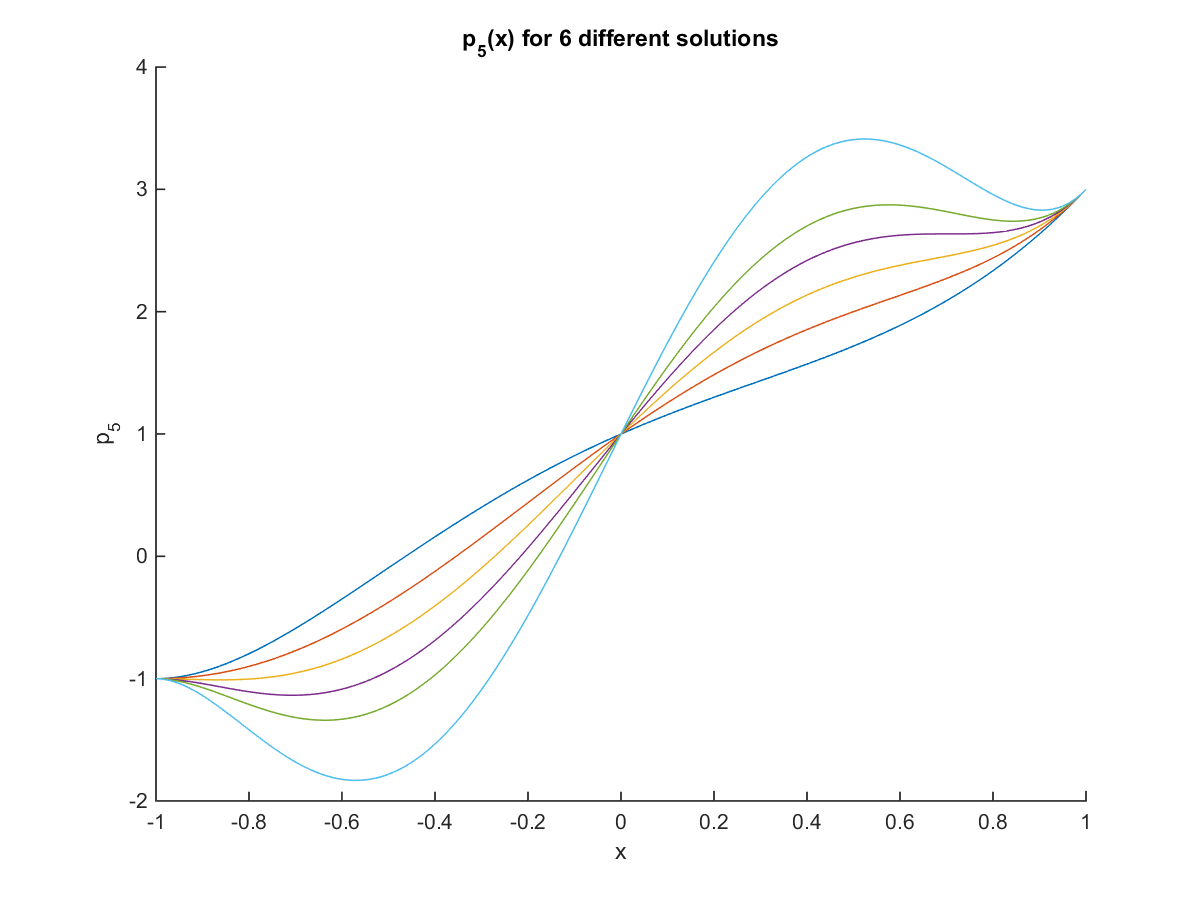
\includegraphics[scale=0.8]{p5_6solutions.png}
			\caption{Polynomial of $p_5$ with 6 different solutions}
		\end{figure}
	\end{enumerate}
		
\large\textbf{Problem 3.} The \textit{Hermite interpolant} $h_n \in \mathcal{P}_{2n+1}$ of $f \in C^1[a,b]$ at the points $\{x_j\}_{j=0}^n$ can be written in the form: 
	\hspace*{3cm} $$h_n(x) = \sum_{j=0}^{n}(A_j(x)f(x_j) + B_j(x)f'(x_j))$$
	where the functions $A_j$ and $B_j$ generalize the Lagrange basis functions:\\
	\hspace*{3cm} $ A_j(x) = (1-2l'_j(x_j)(x - x_j))l_j^2(x)$ \\
	\hspace*{3cm} $ B_j(x) = (x - x_j)l_j^2(x)$ \\
	with $l_j = \prod_{k=0, k \neq j}^{n} (x-x_k)/(x_j-x_k) $
	\begin{enumerate}
		\item Verify that: \\
		$A_j(x_k) = \begin{cases} 1 & \quad j = k \\ 0 & \quad j \neq k 	\end{cases} $ \hspace{0.5cm} $A'_j(x_k) = 0$ \hspace{0.5cm} $B_j(x_k) = 0$ \hspace{0.5cm} $B'_j(x_k) = \begin{cases}
		1 & \quad j = k  \\ 0 & \quad j \neq k 
		\end{cases} $ \\
		As Lagrange basis function: \\
		$\bullet$ if $k \neq j$ then $l_j(x_k) =0 \Rightarrow \begin{cases}  A_j(x_k) = 0 \\ B_j(x_k) = 0 \end{cases} $\\
		$\bullet$ if $k = j$ then $\begin{cases} l_j(x_k) = 1 \\ x_k - x_j = xj - x_j = 0 \end{cases} \Rightarrow \begin{cases} A_j(x_j) = 1 \\ B_j(x_j) = 0 \end{cases} $ \\
		as a result: \hspace{0.5cm} $A_j(x_k) = \begin{cases} 1 & \quad j = k \\ 0 & \quad j \neq k 	\end{cases} $ \hspace{0.5cm} and \hspace{0.5cm} $B_j(x_k) = 0$ \hspace{0.3cm}   $\forall j,k$ \\
		
		$ \textbf{A}'_j(x) = -2l'_j(x_j)l_j^2(x) + 2[1-2l'_j(x_j)(x-x_j)]l'_j(x)l_j(x)$\\
		\hspace*{1cm} $\bullet$ if $k \neq j \Rightarrow l_j(x_k) = 0 $:\\
		\hspace*{2.5cm} $\Rightarrow A'_j(x_k) = -2l'_j(x_j).0^2 + 2[1-2l'_j(x_j)(x_k-x_j)]l'_j(x_k).0 =0$\\
		\hspace*{1cm} $\bullet$ if $k = j \Rightarrow A'_j(x_j) = -2l'_j(x_j)l_j^2(x_j) + 2[1-2l'_j(x_j)(x_j-x_j)]l'_j(x_j)l_j(x_j)$\\
		\hspace*{4.65cm} $ = -2l'_j(x_j) + 2l'_j(x_j)$ \hspace{0.5cm}(because $l_j(x_j)=1$) \\
		\hspace*{4.65cm} $ = 0$ \\
		\hspace*{1.5cm} $ \Rightarrow A'_j(x) = 0$ \hspace{0.3cm} $\forall j,k$
		
		$\textbf{B}'_j(x) = l_j^2(x) + 2(x-x_j)l'_j(x)l_j(x)$ \\
		\hspace*{1cm} $\bullet$ if $k \neq j \Rightarrow l_j(x_k) = 1 \Rightarrow B'_j(x) = 1^2 + 2(x_j-x_j).l'_j(x_j).1 = 1$ \\
		\hspace*{1cm} $\bullet$ if $k \neq j \Rightarrow l_j(x_k) = 0 \Rightarrow B'_j(x) = 0^2 + 2(x_k-x_j)l'_j(x_k).0=0 $ \\
		\hspace*{1.5cm} $ \Rightarrow B'_j(x_k) = \begin{cases} 1 & \quad j = k  \\ 0 & \quad j \neq k 	\end{cases} $ \\
		
		\item The above expression for the Hermite interpolating polynomial mimics the \textit{Lagrange form} of the standard interpolating polynomial. Devise a scheme for constructing Hermite interpolants the generalizes the \textit{Newton form}. What are your Newton-like basis function for $\mathcal{P}_{2n+1}$? \\
		
		First consider: \\
		$\lim_{x \to x_0} f[x_0,x] = \lim_{x \to x_0} \dfrac{f(x) - f(x_0)}{x-x_0} = f'(x_0)$\\
		This motivates the notation: $f[x_0,x_0] = f'(x_0)$\\
		Using the identity: $ f[x_0,x_1,...,x_k] = \dfrac{1}{k!}f^{(k)}(\xi)$ , $\xi \in (x_0,x_k)$ \\
		we have: $f[x_0,...,x_0] = \dfrac{1}{k!}f^{(k)}(x_0)$ \\
		We can form:
		\hspace*{2cm} $$p(x) = \sum_{j=0}^{n}f[x_0,..,x_j]\prod_{i=0}^{j-1}(x-x_i)$$
	\end{enumerate}
	 

\large\textbf{Problem 4.} The one-dimensional interpolation scheme studied in class can be adapted to higher dimensions. For example, suppose we are given a scalar-valued function $f(x,y)$, such as: \\
	\hspace*{3cm} $f(x,y) = e^xsiny$ \\
	and wish to construct a function of the form: \\
	\hspace*{3cm} $p(x,y) = c_0 + c_1x + c_2y + c_3xy + c_4x^2 + c_5y^2$
	that interpolates $f(x,y)$ at $(x_0,y_0), (x_1, y_1), (x_2, y_2), (x_3, y_3), (x_4, y_4), (x_5, y_5)$. 
	\begin{enumerate}
		\item Set up a linear system \textbf{Ac = f} to determine the coefficients $c_0, ..., c_5$.\\
		Based on interpolate points we form 6 different equations:\\
		$p(x_0,y_0) = c_0 + c_1x_0 + c_2y_0 + c_3x_0y_0 + c_4x_0^2 + c_5y_0^2 = f(x_0,y_0) = e^{x_0}\sin {y_0}$ \\
		$p(x_1,y_1) = c_0 + c_1x_1 + c_2y_1 + c_3x_1y_1 + c_4x_1^2 + c_5y_1^2 = f(x_1,y_1) = e^{x_1}\sin {y_1}$ \\
		$p(x_2,y_2) = c_0 + c_1x_2 + c_2y_2 + c_3x_2y_2 + c_4x_2^2 + c_5y_2^2 = f(x_2,y_2) = e^{x_2}\sin {y_2}$ \\
		$p(x_3,y_3) = c_0 + c_1x_3 + c_2y_3 + c_3x_3y_3 + c_4x_3^2 + c_5y_3^2 = f(x_3,y_3) = e^{x_3}\sin {y_3}$ \\
		$p(x_4,y_4) = c_0 + c_1x_4 + c_2y_4 + c_3x_4y_4 + c_4x_4^2 + c_5y_4^2 = f(x_4,y_4) = e^{x_4}\sin {y_4}$ \\
		$p(x_5,y_5) = c_0 + c_1x_5 + c_2y_5 + c_3x_5y_5 + c_4x_5^2 + c_5y_5^2 = f(x_5,y_5) = e^{x_5}\sin {y_5}$ \\
		We have the linear system:\\
		$\textbf{Ac} = \textbf{f} \Leftrightarrow \begin{bmatrix} 1&x_0&y_0&x_0y_0&x_0^2&y_0^2 \\ 1&x_1&y_1&x_1y_1&x_1^2&y_1^2 \\ 1&x_2&y_02&x_2y_2&x_2^2&y_2^2 \\ 1&x_3&y_3&x_3y_3&x_3^2&y_3^2 \\ 1&x_4&y_4&x_4y_4&x_4^2&y_4^2 \\ 1&x_5&y_5&x_5y_5&x_5^2&y_5^2 \end{bmatrix} \begin{bmatrix} c_0\\c_1\\c_2\\c_3\\c_4\\c_5 \end{bmatrix} = \begin{bmatrix} e^{x_0}\sin y_0 \\ e^{x_1}\sin y_1 \\ e^{x_2}\sin y_2 \\ e^{x_3}\sin y_3 \\ e^{x_4}\sin y_4 \\ e^{x_5}\sin y_5 \end{bmatrix} $ \\
		
		
		\item Write a MATLAB code to determine \textbf{c} when $f\{x,y\} = e^x\sin y$ and the $(x_j,y_j)$ pairs take the values listed in the following table.
			\begin{center}
				\begin{tabular} {| c | c | c | c | c | c | c |}
					 \hline
					j & 0 &1 &2 &3 &4 &5 \\
					\hline
					$x_j$ & 0& 0&1&1&2&2 \\
					\hline
					$y_j$ & 0&2&0&2&1&3\\
					\hline
				\end{tabular}
			\end{center}
		Based on the provided interpolant points we can rewrite above function \textbf{Ac = f} as follow: \\
		\hspace*{2cm} $\textbf{Ac} = \textbf{f} \Leftrightarrow \begin{bmatrix} 1&0&0&0&0&0 \\ 1&0&2&0&0&4 \\ 1&1&0&0&1&0 \\ 1&1&2&2&1&4 \\ 1&2&1&2&4&1 \\ 1&2&3&6&4&9 \end{bmatrix} \begin{bmatrix} c_0\\c_1\\c_2\\c_3\\c_4\\c_5 \end{bmatrix} = \begin{bmatrix} 0 \\ 0.9093 \\ 0 \\ 2.472 \\ 6.2177 \\ 1.043 \end{bmatrix} $ \\
	%	Applied MATLAB to solve this equations:
		\begin{lstlisting}
% Determine c based on interpolant points
A = [1,0,0,0,0,0; 1,0,2,0,0,4; 1,1,0,0,1,0; 1,1,2,2,1,4; ... 
     1,2,1,2,4,1; 1,2,3,6,4,9];
B = [0;0.9093;0;2.472;6.2177;1.043];
c = linsolve(A,B);
		\end{lstlisting}
		\begin{lstlisting}
			>> c
					c =
							0
							-0.9490
							5.0593
							0.7813
							0.9490
							-2.3023
		\end{lstlisting}
		
		
		\item Plot your model function $p(x,y)$ over $x \in [-1, 3], y \in [-1,3]$ using $\mathtt{MATLAB's}$ $\mathtt{surf}$ command.\\
		Compare this plot to the similar plot for $f(x,y)$, which can be obtained in the following manner. 
		\begin{lstlisting}
% Plot from function f(x,y)
f = inline('exp(x).*sin(y)','x','y');
[xx,yy] = meshgrid(linspace(-1,3,25),linspace(-1,3,25));
zz = f(xx,yy);
figure(1), clf
surf(xx,yy,zz);
title('f(x,y)'); print('f_xy','-dpng');
%Plot from funtion p(x,y)
p = @(x,y) c(1,1) + c(2,1)*x + c(3,1)*y + c(4,1)*x.*y ...
     + c(5,1)*x.^2 + c(6,1)*y.^2;
pp = p(xx,yy);
figure;
surf(xx,yy,pp);
title('p(x,y)'); print('p_xy','-dpng');
		\end{lstlisting}
		
		\begin{figure}[htp]
			\begin{center}
				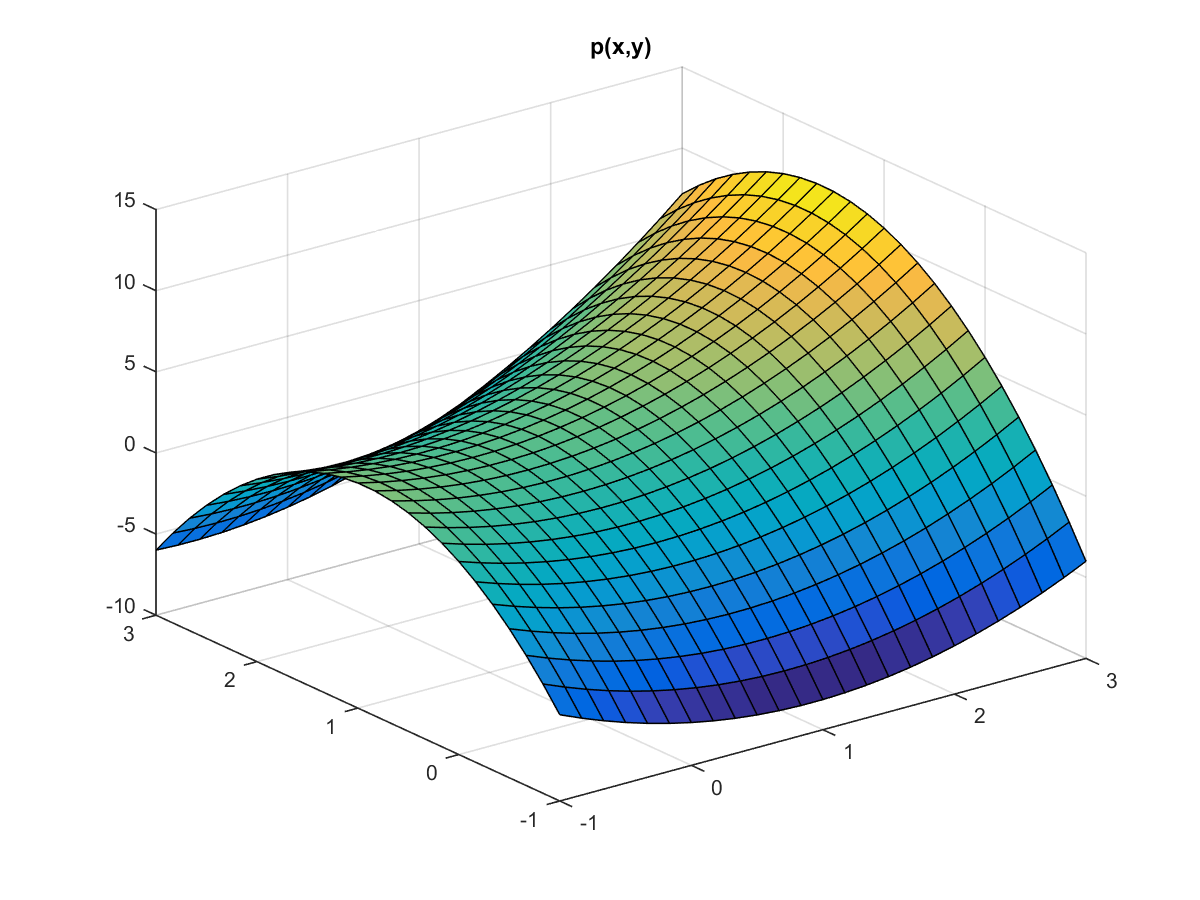
\includegraphics[scale=0.6]{p_xy.png}
				\caption{$p(x,y)$ plot with $\mathtt{surf}$ over $x \in [-1,3], y\in [-1,3]$}
			\end{center}
		\end{figure}
		\pagebreak
		\begin{figure}[htp]
			\begin{center}
				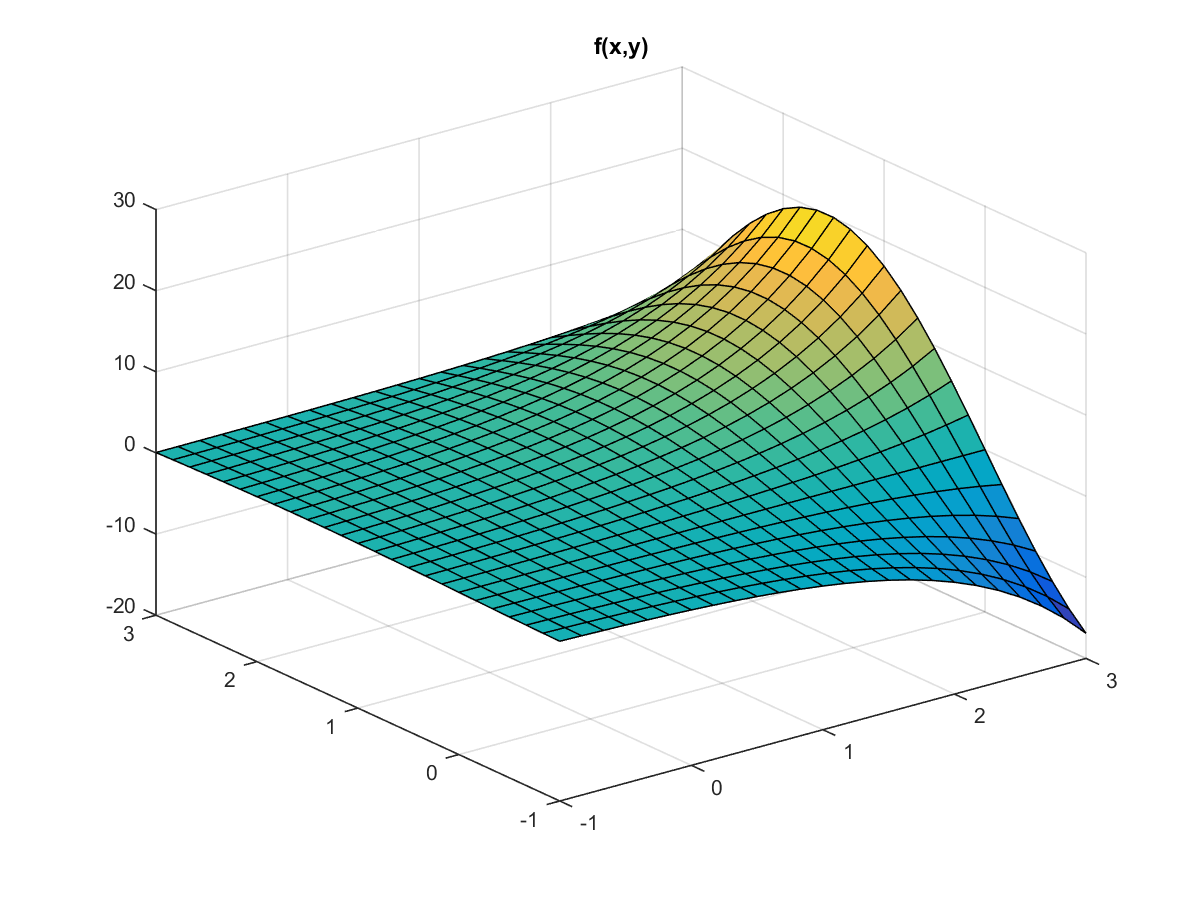
\includegraphics[scale=0.6]{f_xy.png}
				\caption{$f(x,y)$ plot with provided function}
			\end{center}
		\end{figure}
		
		 
	\end{enumerate}	 

\large\textbf{Problem 6.} The standard Lagrange interpolation formula for the polynomial $p_n \in \mathcal{P}_n$ that interpolates $f \in C[a,b]$ at the distinct points $\{x_j\}$: 
	$$p_n(x) = \sum_{j=0}^{n}l_j(x)f(x_j), \hspace{0.5cm} where \hspace{0.3cm} l_j = \prod_{k=0, k \neq j}^{n}\dfrac{(x-x_k)}{(x_j-x_k)} $$ 
	require $O(n^2)$ floating point operations to evaluate for each point $x$. In this exercise, we construct an alternative Lagrange interpolation formula, known as the \textit{barycentric interpolant}, that can evaluated more efficiently and also has superior numerical stability.\\
	Let $$w(x) = \prod_{k=0}^{n}(x-x_k)$$ and define the \textit{barycentric weight} as: \hspace{1cm} $\beta_j = \dfrac{1}{\prod_{k=0,k \neq j}^{n}(x-x_j)}$, $j = 0, ..., n$
	\begin{enumerate}
		\item Based of above definitions, the Lagrange form for $p_n$ can be rewritten as:
		 $$p_n(x) = \sum_{j=0}^{n}l_j(x)f(x_j) = \sum_{j=0}^n \left( \prod_{k=0, k \neq j}^{n}\dfrac{(x-x_k)}{(x_j-x_k)} f(x_j)\right) $$ 
		 \hspace*{4cm} $$ = \sum_{j=0}^n \left( \prod_{k=0, k \neq j}^{n}(x-x_k) \prod_{k=0, k \neq j}^{n}\dfrac{1}{(x_j-x_k)}f(x_j) \right)$$
		 \hspace*{4cm} $$ = \sum_{j=0}^n \left(\left( \prod_{k=0}^{n}(x-x_k) \right) \dfrac{1}{x-x_j}\beta_jf(x_j) \right)$$
		 \hspace{4cm} $$ = \sum_{j=0}^n w(x) \dfrac{\beta_j}{(x-x_j)}f(x_j) $$
		 \hspace{4cm} $$ = w(x)\sum_{j=0}^n  \dfrac{\beta_j}{(x-x_j)}f(x_j) $$
		
		
		\item Verify that: \hspace{1cm} $$ 1 = w(x)\sum_{j=0}^{n} \dfrac{\beta_j}{x-x_j}$$
		Belong to above expression we have: $l_j(x) = w(x).\dfrac{\beta_j}{x-x_j}$
		$$ \Rightarrow \sum_{j=0}^{n}l_j(x) = \sum_{j=0}^{n} w(x)\dfrac{\beta_j}{x-x_j} = w(x) \sum_{j=0}^{n}\dfrac{\beta_j}{x-x_j}$$
		Besides, based on definition of Lagrange basis function: $$\begin{cases} l_j(x_k) = 0 & \quad j \neq k \\ l_j(x_k) = 1 & \quad j = k \end{cases} \Rightarrow \sum_{j=0}^{n} l_j(x) = 1$$ 
		From 2 above equations we can affirm that: $$ 1 = w(x)\sum_{j=0}^{n} \dfrac{\beta_j}{x-x_j}$$
		Or by choosing $f(x) = 1$ we also have the same result.
		
		\item Dividing the result of part (a) by the result of part (b) yields the \textit{barycentric interpolation formular}:\\
		\hspace*{2cm} $ p_n(x) = \dfrac{\sum_{j=0}^{n}\dfrac{\beta_j}{x-x_j}f(x_j)}{\sum_{j=0}^{n}\dfrac{\beta_j}{x-x_j}} $ \\
		Assuming the $\beta_j$ values are already known, in order to evaluate $p_5$ we will need $O(n)$ floating point operations:
		
		For the numerator each $j$ value we have $3(n+1)$ operations ($2(n+1)$ for 2 times of $(x-x_j)$ and one time for $f(x_j)$). \\
			For the denominator we need $n$ operations\\ 
			$\Rightarrow$ in total we need $4n + 3$ operations = $O(n)$. 
						
		\item Suppose $[a,b] = [0,1]$ and $x_j = j/n$ for $j = 0, ..., n$. Derive a simple formula for $\beta_j$ in terms of $j$ and $n$: \\
		Replaced $x_j$ into definition of the \textit{barycentric weight} we have:\\
		$\beta_j = \dfrac{1}{\prod_{k=0,k \neq j}^{n}(\dfrac{j}{n}-\dfrac{k}{n})} = \dfrac{1}{\dfrac{1}{n^n}\prod_{k=0,k \neq j}^{n}(j-k)} =\dfrac{n^n}{\prod_{k=0,k \neq j}^{n}(j-k)}  = \dfrac{n^n}{j!(n-j)!}$ \\
	
		$\beta_j$ get the largest value when $g(j) = j!(n-j)!$ hit the smallest value. We have:\\
		Assume that $n$ is a even number, we'll make a comparison between $g(\dfrac{n}{2})$ and $g(\dfrac{n}{2}+1)$:\\
		\hspace*{2cm} $\dfrac{g(\dfrac{n}{2})}{g(\dfrac{n}{2}+1)} = \dfrac{\dfrac{n}{2}!\dfrac{n}{2}!}{(\dfrac{n}{2}-1)!(\dfrac{n}{2}+1)!} = \dfrac{\dfrac{n}{2}}{\dfrac{n}{2}+1} < 1$ \\
		$\Rightarrow \beta_j$ largest at $j =\dfrac{n}{2}$: $\beta_j = \dfrac{n^n}{\dfrac{n}{2}!\dfrac{n}{2}!} = \dfrac{4n^n}{(n!)^2} $ \\
		
		In case $n$ is a odd number, follow the same step, we could proof that the highest value of $\beta_j$ at $ceil(\dfrac{n}{2})$ or $floor(\dfrac{n}{2})$.
		
	\end{enumerate} 
	
\end{document}